\section{积分与极限的交换}
\label{sec:ru-limit-interchange}

用函数列逼近被积函数时，自然希望积分也随之收敛，即$\lim\int f_n=\int\lim f_n$。这是交换“积分”与“取极限”两个操作，和交换求导与极限一样，需要条件。

\subsection{函数列、级数与逐项积分}
\label{sec:ru-termwise-integration}

在固定的闭区间上，一致收敛足以保证交换。
\begin{theorem}[一致收敛与积分]
\label{thm:ru-uniform-limit-integral}
设每个$f_n$在$[a,b]$上黎曼可积，且$f_n$在$[a,b]$上一致收敛到$f$，则$f$在$[a,b]$上黎曼可积，并且$\int_a^bf_n\to\int_a^bf$。
\end{theorem}
\begin{proof}
给定$\varepsilon>0$，取$n$使$|f_n-f|<\varepsilon$处处成立。在每一小段上，$f$的上下确界与$f_n$的相差不超过$\varepsilon$，所以$U(f,P)-L(f,P)\leq U(f_n,P)-L(f_n,P)+2\varepsilon(b-a)$，
再取使$f_n$的上下和之差小于$\varepsilon$的分割，由Darboux判据$f$可积。积分的收敛来自误差估计：$\bigl|\int_a^bf_n-\int_a^bf\bigr|\leq(b-a)\sup_{[a,b]}|f_n-f|\to0$。
\end{proof}
证明的关键是“统一误差乘以区间长度”，所以区间必须有限，误差必须对所有$x$统一。逐点收敛不够，下面的窄峰说明了原因。
在$[0,1]$上令$f_n$在$[0,2/n]$上是以$(1/n,n)$为顶点的三角形，其余处为零（$n\geq2$）。每个三角形的面积都是$1$，所以$\int_0^1f_n=1$；
但对每个$x$，$f_n(0)=0$，而$x>0$时一旦$2/n<x$就有$f_n(x)=0$，所以$f_n$逐点收敛到$0$，积分的极限$1$不等于极限函数的积分$0$。
如图~\ref{fig:ru-narrow-spikes}所示，尖峰越来越窄、越来越高，总面积不变，却躲开了每一个固定的点；最大误差$\sup|f_n-0|=n$并不趋于零。

\begin{figure}[!htbp]
 \centering
 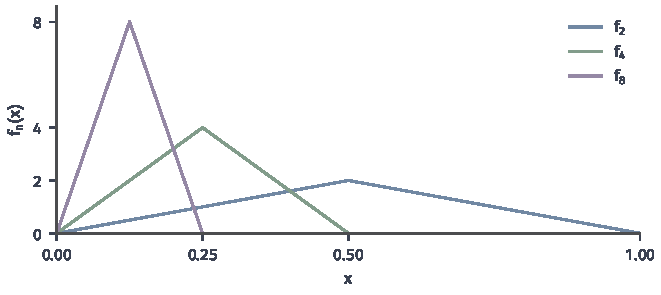
\includegraphics[width=112mm]{figures/01-mathematical-preliminaries-upper/02-real-numbers-and-univariate-functions/matplotlib/narrow-spikes/figure.pdf}
 \caption{窄峰函数列：$f_n$在$[0,2/n]$上为顶点$(1/n,n)$的三角形，其余处为零，图中画出$n=2,4,8$。每个三角形面积为$1$；固定任一$x>0$，$n>2/x$后$f_n(x)=0$，所以$f_n$逐点趋于零，积分却始终为$1$。图为解析示例。}
 \label{fig:ru-narrow-spikes}
\end{figure}

把定理用于部分和：若各项$g_k$在$[a,b]$上可积，$\sum g_k$在$[a,b]$上一致收敛，则可以逐项积分，$\int_a^b\sum g_k=\sum\int_a^bg_k$。
幂级数在收敛区间内部的闭子区间上一致收敛，所以对$|x-x_0|<R$，
\[
 \int_{x_0}^x\sum_kc_k(t-x_0)^k\,\mathrm dt=\sum_k\frac{c_k}{k+1}(x-x_0)^{k+1},
\]
逐项积分后的级数仍以$R$为收敛半径。由几何级数$\frac1{1-t}=\sum t^k$（$|t|<1$），在$[0,x]$上逐项积分得
\[
 -\log(1-x)=\sum_{k=1}^\infty\frac{x^k}k,\qquad|x|<1.
\]
这兑现了第~\ref{sec:ru-power-series-uniform}节的说法：右边的级数在$x=-1$处收敛，和函数在$[-1,1)$上连续；左边也在$x=-1$处连续，两者在$(-1,1)$上相等，在$-1$处也相等，于是$\log2=1-\frac12+\frac13-\cdots$。
同样，由$\frac1{1+t^2}=\sum(-1)^kt^{2k}$逐项积分得$\arctan x=\sum(-1)^k\frac{x^{2k+1}}{2k+1}$（$|x|<1$），右边在$x=1$处由Leibniz判别收敛，再用Abel第二定理得到$\frac\pi4=1-\frac13+\frac15-\cdots$。
这些结论都在有限闭区间上取得，不能直接推广为反常积分上的无条件交换：反常积分还多了一次截断的极限，需要另外控制。

\subsection{含参积分的连续与求导}
\label{sec:ru-parametric-integrals}

被积函数含有一个参数$y$时，积分$F(y)=\int_a^bf(x,y)\,\mathrm dx$是$y$的函数，称为含参积分。这里积分区间固定且有限，参数是唯一变化的实数。
$F$在$y_0$处是否连续，就是能否交换$y\to y_0$与积分。由上一小节的误差估计，若$y\to y_0$时$f(\cdot,y)$关于$x$一致趋于$f(\cdot,y_0)$，即$\sup_{x\in[a,b]}|f(x,y)-f(x,y_0)|\to0$，则$|F(y)-F(y_0)|\leq(b-a)\sup_x|f(x,y)-f(x,y_0)|\to0$，$F$在$y_0$处连续。
只在每个$x$处控制是不够的。把窄峰改写成连续参数：$y>0$时令$f(\cdot,y)$为$[0,2y]$上以$(y,1/y)$为顶点的三角形，$f(\cdot,0)\equiv0$。
对每个$x$，$y\to0^+$时$f(x,y)\to0$，但$y\leq1/2$时$F(y)=1$，而$F(0)=0$，$F$在$0$处不连续。

对参数求导也是一种极限交换。固定$x$，考察参数的差商$D_h(x)=[f(x,y+h)-f(x,y)]/h$，则$[F(y+h)-F(y)]/h=\int_a^bD_h(x)\,\mathrm dx$。
\begin{theorem}[积分号下求导]
\label{thm:ru-differentiation-under-integral}
设对$y$附近的每个参数，$f(\cdot,y)$在$[a,b]$上黎曼可积；并且$h\to0$时，$D_h$在$[a,b]$上一致收敛到某个函数$g$。则$F$在$y$处可导，且$F'(y)=\int_a^bg(x)\,\mathrm dx$。
\end{theorem}
\begin{proof}
任取一列$h_n\to0$，$D_{h_n}$在$[a,b]$上可积且一致收敛到$g$，由定理~\ref{thm:ru-uniform-limit-integral}，$g$可积且$\int D_{h_n}\to\int g$。由序列判据，差商$[F(y+h)-F(y)]/h\to\int g$。
\end{proof}
若$f$关于$y$可导，极限函数$g$就是偏导数$\partial f/\partial y$在$y$处的值，定理说的是$F'(y)=\int_a^b\frac{\partial f}{\partial y}(x,y)\,\mathrm dx$在差商一致收敛时成立。
以$F(y)=\int_0^1e^{xy}\,\mathrm dx$为例，参数只出现在指数因子中。由第~\ref{sec:ru-elementary-limits}节的估计$|e^u-1-u|\leq2u^2$（$|u|<1/2$），
\[
 \Bigl|D_h(x)-xe^{xy}\Bigr|=e^{xy}\Bigl|\frac{e^{xh}-1-xh}h\Bigr|\leq2e^{|y|}|h|,\qquad x\in[0,1],\ |h|<\tfrac12,
\]
所以差商关于$x$一致收敛，$F'(y)=\int_0^1xe^{xy}\,\mathrm dx$。$y\neq0$时可以直接核对：$F(y)=(e^y-1)/y$，两边都等于$(ye^y-e^y+1)/y^2$。
实际应用中更方便的充分条件是偏导数关于$(x,y)$连续，它需要多元函数的连续性，留到多元函数微积分部分（第~\ref{chap:multivariate-calculus}章）。
